%		For public use only, fair use laws still apply
%		A tutorial template created by Chad Gibbons




%	I recommend for generic help the following website
%	http://www.emerson.emory.edu/services/latex/latex_toc.html
%	There are many good websites and forums for LaTeX
%
%	If you have a problem, google it. (ex. "How do I start my page numbers at a different number")



%%%%%%%%%%%%%%%%%%%%%%%%%%%%%%%%%%%%%%%%%%%%%%%%%%%%%%
%					 													  %
%					 													  %
%					  ALWAYS BEGIN THE PROGRAM WITH								  %
%					 													  %
%						\documentclass{class_type}								  %
%																		  %
%		Different class types have different commands associated with them, similar to header files			  %
%					 													  %
%					 													  %
%%%%%%%%%%%%%%%%%%%%%%%%%%%%%%%%%%%%%%%%%%%%%%%%%%%%%%

\documentclass{article}

%%%%%%%%%%%%%%%%%%%%%%%%%%%%%%%%%%%%%%%%%%%%%%%%%%%%%%
%					 													  %
%					 													  %
%				It is recommended to only use packages as you need them 						  %
%					 													  %
%	Different types of reports will consistently use specific packages; keep these in their respective templates		  %
%					 													  %
%					 													  %
%%%%%%%%%%%%%%%%%%%%%%%%%%%%%%%%%%%%%%%%%%%%%%%%%%%%%%


\usepackage{babel}				%	Expands text mode
\usepackage{csquotes}				%	Permits \enquote{quote}
\usepackage{graphicx}				%	Permits \includegraphics[]{image}
\usepackage{caption}				%	Permits the void caption \caption*{}
\usepackage{a4wide}				%	Expands width of body

\usepackage{epstopdf}				% 	Three Lines of Code permit usage of .tif images
\epstopdfDeclareGraphicsRule{.tif}{png}{.png}{convert #1 \OutputFile}
\AppendGraphicsExtensions{.tif}


%%%%%%%%%%%%%%%%%%%%%%%%%%%%%%%%%%%%%%%%%%%%%%%%%%%%%%%			PREAMBLE


\title{Image Processing \\ Mini Project 1 \\Dr. Ononye}		%note left quote command vs " = \textquotedblright
\author{Gibbons, Chad  \\ Glass, Benjamin  \\ Rodriguez, Angel }
%\date{02/15/2019}					%	Set permanent date or use date section as additional text real estate on the title page.
%\date{Sic et Non \\ Quid Faciendus Est}



%%%%%%%%%%%%%%%%%%%%%%%%%%%%%%%%%%%%%%%%%%%%%%%%%%%%%%%			DOCUMENT





%%%%%%%%%%%%%%%%%%%%%%%%%%%%%%%%%%%%%%%%%%%%%%%%%%%%%%
%					 													  %
%					 													  %
%					  ALWAYS BEGIN THE DOCUMENT WITH								  %
%					 													  %
%							\begin{document}									  %
%					 													  %
%					 													  %
%%%%%%%%%%%%%%%%%%%%%%%%%%%%%%%%%%%%%%%%%%%%%%%%%%%%%%


\begin{document}

\maketitle

	%%%%%%%%%%%%%%%%%%%%%%%%%%%%%%%%%%%%%%%%%%
	%														 %
	%														 %
	%		\hfill fills in the remaining spaces of the given line with spaces			 %
	%														 %
	%					\\ ends line           							 %
	%														 %
	%	Determine the number of "\hfill \\ " iterations in accord with the number of lines		 %
	%				   within you abstract.							 %
	%														 %
	%														 %
	%%%%%%%%%%%%%%%%%%%%%%%%%%%%%%%%%%%%%%%%%%

\hfill 
\hfill \\
\hfill \\
\hfill \\
\hfill \\
\hfill \\
\hfill \\
\hfill \\
\hfill \\
\hfill \\
\hfill \\
\hfill \\
\hfill \\
\hfill \\
\hfill \\
\hfill \\
\hfill \\
\hfill \\
\hfill \\
\hfill \\
\hfill \\
\hfill


	%%%%%%%%%%%%%%%%%%%%%%%%%%%%%%%%%%%%%%%%%%
	%														 %
	%														 %
	%		The primary purpose of an abstract is to give sufficient information		 %
	%					on your report to inform 						 %
	%		researchers, students, grant providers, corporate executives, professors,  	 %
	%				professionals, or the audience of your intention			 %
	%		whether or not either reading or purchasing your report is necessary.		 %
	%														 %
	%														 %
	%%%%%%%%%%%%%%%%%%%%%%%%%%%%%%%%%%%%%%%%%%

\begin{abstract}
\noindent
This document presents both the target and duplicated images with minimal commentary. \\ 
Detailed information can be found in the project's .m (MATLAB) file.
\end{abstract}

\pagenumbering{gobble}

%\pagebreak


%\tableofcontents



	%%%%%%%%%%%%%%%%%%%%%%%%%%%%%%%%%%%%%%%%%%
	%														 %
	%														 %
	%		\pagenumbering{gobble}	"gobbles" or removes the pagination of the page  	 %
	%					and the following pages.						 %
	%														 %
	%		\pagenumbering{num_style}	sets the pagination of the page and 	  	 %
	%						the following pages						 %
	%														 %
	%						{num_style} List:						 %
	%														 %
	%				{roman} -> lowercase roman numerals           				 %
	%				{Roman} -> uppercase roman numerals           				 %
	%				{alph} -> lowercase alphabetical numerals           			 %
	%				{Alph} -> uppercase alphabetical numerals           			 %
	%				{arabic} -> standard decimal numerals (0-9)           			 %
	%														 %
	%			Altering \pagenumbering{} will restart the pagination at 1.			 %
	%			     See other tutorial for greater control of paginations.			 %
	%														 %
	%														 %
	%%%%%%%%%%%%%%%%%%%%%%%%%%%%%%%%%%%%%%%%%%


%\pagenumbering{roman}

\pagebreak

\section{Figure Analysis pg. 72}

\begin{figure}[h!]
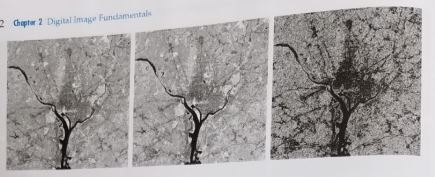
\includegraphics[scale=1.25]{pg72.jpg}
\caption{Images on page 72 to match}
\end{figure}

\noindent
The middle image is the result from setting the image's least significant bit of every pixel to zero.\\
The right image is the result of the difference between the two images.\\
The original image on the left is courtesy of NASA.\\



\section{Figure Analysis pg. 79}


\begin{figure}[h!]
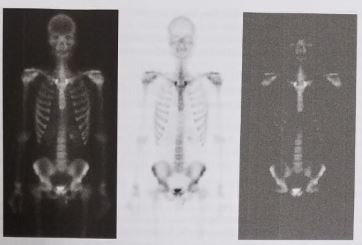
\includegraphics[scale=1.0]{pg79.jpg}
\caption{Images on page 79 to match}
\end{figure}

\noindent
Left image is original.\\
Center image is negative of original.\\
Right image is the union of the other images.\\
The union of two grayscale sets A and B with the same number of elements is defined as the set.\\
$$
A \Upsilon B = \Bigg\{ max(a,b) \big| a \epsilon A, b \epsilon B \Bigg\}
$$


\section{Figure Analysis pg. 137}


\begin{figure}[h!]
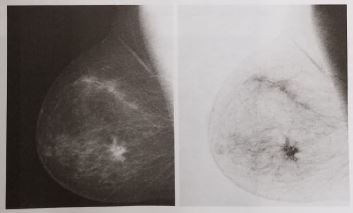
\includegraphics[scale=1.0]{pg137.jpg}
\caption{Images on page 137 to match}
\end{figure}

\noindent 
Left image is original.\\
Right image is negative of original. \\


\section{Figure Analysis pg. 140}



\begin{figure}[h!]
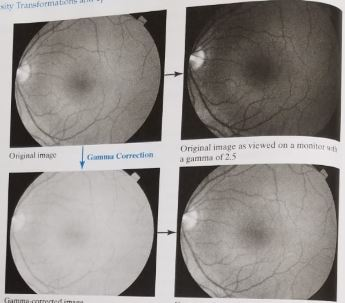
\includegraphics[scale=1.0]{pg140.jpg}
\caption{Images on page 140 to match}
\end{figure}

\noindent
Upper left image is original.\\
Upper right image is gamma set to 2.5 of original image.\\
Lower left image is gamma-corrected image.\\
Lewer right image is the returning of the gamma-corrected image to monitor image.\\
Image courtesy of Nation Eye Institute.\\


\section{Figure Analysis pg. 142}



\begin{figure}[h!]
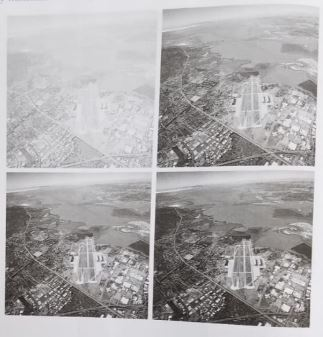
\includegraphics[scale=1.0]{pg142.jpg}
\caption{Images on page 142 to match}
\end{figure}

\noindent
Upper left image is original with noise.\\
Upper right image is presented with $\gamma$ = 3.0.\\
Lower left image is presented with $\gamma$ = 4.0.\\
Lower right image is presented with $\gamma$ = 5.0.\\
Image courtesy of NASA.\\



	%%%%%%%%%%%%%%%%%%%%%%%%%%%%%%%%%%%%%%%%%%
	%														 %
	%														 %
	%	The primary purpose of an introduction is to provide a fundamental  review		 %
	%				of topics in your report to prepare 					 %
	%		researchers, students, grant providers, corporate executives, professors,  	 %
	%				professionals, or the audience of your intention			 %
	%	with sufficient explanation that someone of appropriate technical knowledge		 %
	%			would be able to comprehend the method and conclusion 			 %
	%														 %
	%														 %
	%%%%%%%%%%%%%%%%%%%%%%%%%%%%%%%%%%%%%%%%%%







	%%%%%%%%%%%%%%%%%%%%%%%%%%%%%%%%%%%%%%%%%%
	%														 %
	%														 %
	%					Special Note on Quotation Marks					 %
	%														 %
	%			   Standard Quotation Mark (") --> right quotation mark			 %
	%			Double Reverse Accent Mark (``) --> left quotation mark	 		 %
	%			left quotation mark = \textquotedblleft vs \textquotedblright 		 %
	%														 %
	%														 %
	%%%%%%%%%%%%%%%%%%%%%%%%%%%%%%%%%%%%%%%%%%



% \section{Table Tutorial}


	%%%%%%%%%%%%%%%%%%%%%%%%%%%%%%%%%%%%%%%%%%
	%														 %
	%														 %
	%					Special Note on Tables						 %
	%														 %
	%				   l = left, c = center, r = right alignment				 %
	%			   | in tabular sets borders between alignment sets		 		 %
	%	      \hline places a horizontal line across width of table above current the line  		 %
	%			   \\ (the endline command) begins next line of table.		 		 %
	%														 %
	%														 %
	%%%%%%%%%%%%%%%%%%%%%%%%%%%%%%%%%%%%%%%%%%


\end{document}




%%%%%%%%%%%%%%%%%%%%%%%%%%%%%%%%%%%%%%%%%%%%%%%%%%%%%%
%					 													  %
%					 													  %
%					  ALWAYS END THE DOCUMENT WITH								  %
%					 													  %
%							\end{document}									  %
%					 													  %
%					 													  %
%%%%%%%%%%%%%%%%%%%%%%%%%%%%%%%%%%%%%%%%%%%%%%%%%%%%%%